\section{Count of 1\'s and 0\'s}
\subsection{Aim}
To count the number of ones and zeros in a binary number

\subsection{Code}
\begin{lstlisting}
DATA SEGMENT
    num DW 0810H
    zeros DW ?
    ones DW ? 
DATA ENDS

CODE SEGMENT
ASSUME CS:CODE, DS:DATA  
START:
    MOV AX, DATA
    MOV DS, AX
    MOV AX, num 
    XOR BX, BX
    XOR CX, CX
SHIFTLOOP:
    SHR AX, 1
    JNC ZERO
    INC BX
    CMP AX, 0
    JNE SHIFTLOOP
    JMP EXIT
ZERO:
    INC CX
    CMP AX, 0
    JNE SHIFTLOOP 
EXIT:
    MOV ones, BX
    MOV zeros, CX
    MOV AH, 4CH
    INT 21H
CODE ENDS
END START
\end{lstlisting}

\subsection{Output}
\begin{center}
	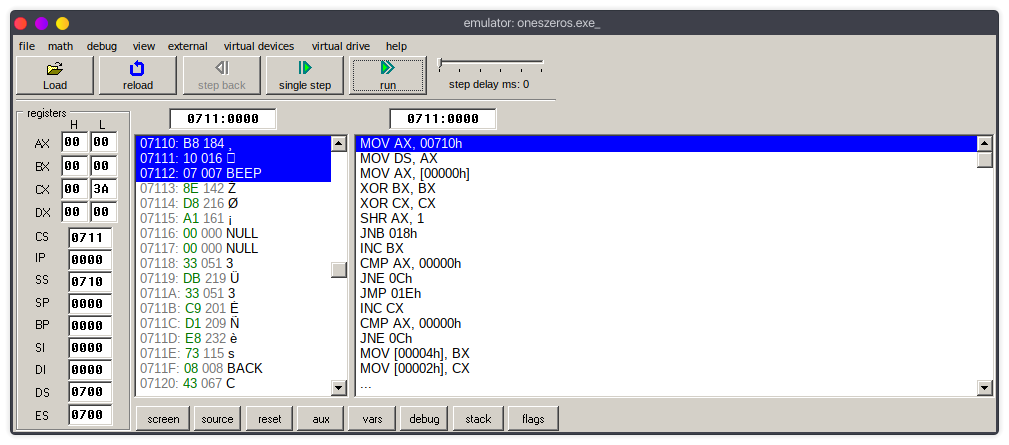
\includegraphics[width=0.90\textwidth]{img/p15/ss1.png}
	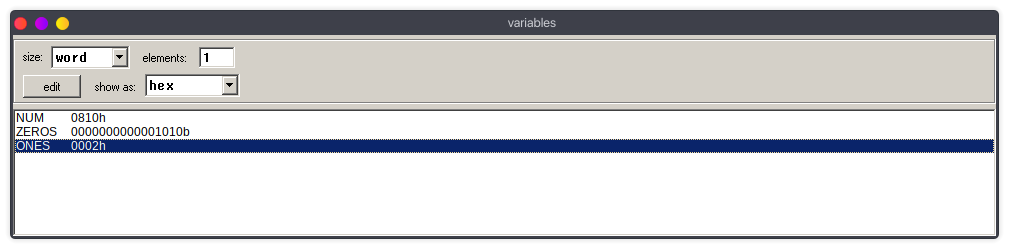
\includegraphics[width=0.90\textwidth]{img/p15/ss2.png}
\end{center}

\subsection{Result}
The number of ones and zeros in a binary number was calculated

